% --------------------------------------------
\documentclass{Arquivos/TrabalhoAcademico} 
% --------------------------------------------
% Dados Pré-Textuais
% --------------------------------------------
\titulo{Monografia:\\ {\large Modelo conforme Normas UFT/ABNT}}
\tituloficha{Monografia: Modelo conforme Normas UFT/ABNT}

\autor{Wenes Aquino}

\orientador{Fulano Aquino Carvalho}
\coorientador{Beltrano Vitória Almeida}

\local{Arraias -- TO}
\data{2025, v-2.0}

\instituicao{%
  Universidade Federal do Tocantins \\
  Campus Universitário de Palmas \\
  Curso de Licenciatura em Computação
}


\tipotrabalho{Trabalho de Conclusão de Curso}


\preambulo{Relatório Técnico apresentado como 
    parte dos requisitos para avaliação na Universidade 
    Federal do Tocantins. Este modelo foi adaptado 
    e personalizado com ajustes visuais e estruturais, 
    servindo também para testar o espaço disponível 
    utilizada nessa contracapa. Por \WenesTex.}



\fichaAssuntos{
 1. Inteligência artificial.
 2. Pensamento computacional.
 3. Computação desplugado.
 I. Orientador.
 II. Universidade Federal do Tocantins.
 III. Campus Universitário de Palmas - Curso de Licenciatura em Computação.
 IV. Título.
}



\begin{document}
\nocite{*}


\pretextual % =================================


\folhaderosto
\contracapa


\fichaCatalografica


\begin{errata}
\noindent Elemento opcional. Deve ser inserida logo após a folha de rosto, constituído pela referência da publicação e pelo texto da errata. Apresentada em papel avulso ou encartado, acrescida ao relatório depois de impresso.\\[1em]

\noindent EXEMPLO:\\[1em]

\noindent ULLER, Leonardo; LOPES, Oswaldo. \textbf{Coordenação de pesquisa sobre corrosão na produção e utilização do álcool}: relatório parcial de 15 de março a 15 de junho de 1982. Rio de Janeiro: FTI, 1982.\\[1em]

\renewcommand{\arraystretch}{1.5}
\begin{center}
    \begin{tabular}{|c|c|l|l|}
        \hline
        Folha & Linha & Onde se lê & Leia-se \\
        \hline
        32 & 3 & publiacao & publicação \\
        \hline
    \end{tabular}
\end{center}
\end{errata}



\folhadeaprovacao


% ===============================================
% -----------------Dedicatória-------------------
% -----------------------------------------------
\begin{dedicatoria}
    Dedicado àqueles que compreendem o valor
    inestimável do conhecimento e da busca incessante
    pela verdade, alicerçando suas conquistas no mérito,
    na responsabilidade individual e na liberdade.
    Que esta jornada científica inspire a próxima
    geração de construtores, movidos pela lógica
    e pela convicção de que o progresso é fruto
    da iniciativa privada e do trabalho honesto.
\end{dedicatoria}
% -----------------------------------------------



\capituloCentralizado*{Agradecimentos}
Elemento opcional. Devem ser inseridos após a errata, se houver.



% ===============================================
% -------------------Epígrafe--------------------
% -----------------------------------------------
\begin{epigrafe}
    ``A verdade é o fundamento que sustenta a mente livre.\\
    Onde há liberdade, nasce a responsabilidade;\\
    onde há responsabilidade, floresce o mérito;\\
    e onde o mérito prevalece, nenhum poder arbitrário\\
    consegue limitar o potencial do indivíduo.\\
    A busca pela liberdade não é apenas um ideal,\\
    mas um compromisso diário com a razão, a coragem\\
    e a defesa daquilo que torna cada ser humano único.''
    
    $\forall$ Libertário - \WenesTex
\end{epigrafe}
% -----------------------------------------------




% ======== RELATÓRIO e TCC ==========%
\begin{resumo}
Este resumo está em conformidade com a \textbf{ABNT NBR 6028:2021}, que estabelece os requisitos para a redação e apresentação de resumos, resenhas e recensões. O resumo é definido como a apresentação concisa dos pontos relevantes de um documento. O texto deve ser composto por uma sequência de \textbf{frases concisas em parágrafo único}, sem enumeração de tópicos. Para trabalhos acadêmicos e relatórios técnicos, como este, recomenda-se a modalidade informativa e a extensão de 150 a 500 palavras. Convém que o texto seja redigido utilizando o \textbf{verbo na terceira pessoa}. As \textbf{palavras-chave} devem figurar logo abaixo do resumo, antecedidas da expressão "Palavras-chave:", \textbf{separadas entre si por ponto e vírgula (;)} e \textbf{finalizadas por ponto (.)}.

\textbf{Palavras-chaves}: ABNT NBR 6028:2021; resumo informativo; parágrafo único; ponto e vírgula; relatório técnico.
\end{resumo}


\begin{resumoEN}

\end{resumoEN}


\listaDeFiguras
\listaDeTabelas


\begin{siglas}
    \item[CPU] Unidade Central de Processamento
    \item[RAM] Memória de Acesso Aleatório
    \item[SSD] Unidade de Estado Sólido (Solid State Drive)
\end{siglas}


\begin{simbolos}
    \item[$\alpha$] Alfa (Ângulo, Coeficiente de Temperatura)
    \item[$\beta$] Beta (Ângulo, Ganho de Corrente do Transistor)
    \item[$\sum$] Somatório (Usado em Séries Matemáticas e Estatística)
\end{simbolos}


\Sumario


\textual % ==================================


\chapter{Introdução}


\part{Preparação} % Opcional 
\chapter{Desenvolvimento}
\section{Desenvolvimento}


\part{Resultado} % Opcional
\chapter{Considerações finais}
\section{Conclusão}


\postextual % ==================================


\capituloCentralizado{Referências}
\printbibliography[heading=none]


\paginaDivisoria{APÊNDICES}
\inicioApendices
\chapter{Apêndice}


\paginaDivisoria{ANEXOS}
\inicioAnexos
\chapter{Anexo}

\begin{table}[ht]
    \centering
    \caption{Tabela estilosa 5×5}
    \label{tab:estilosa}
    \begin{tabular}{ccccc}
        \toprule
        Col 1 & Col 2 & Col 3 & Col 4 & Col 5 \\
        \midrule
        A1 & B1 & C1 & D1 & E1 \\
        A2 & B2 & C2 & D2 & E2 \\
        A3 & B3 & C3 & D3 & E3 \\
        A4 & B4 & C4 & D4 & E4 \\
        A5 & B5 & C5 & D5 & E5 \\
        \bottomrule
    \end{tabular}
\end{table}

\begin{figure}[ht]
    \centering
    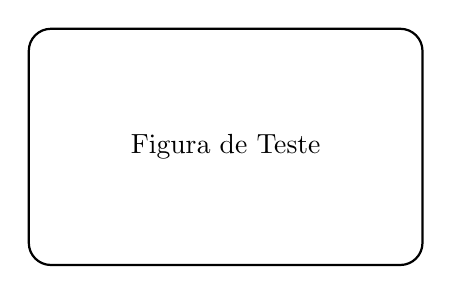
\begin{tikzpicture}
        \draw[rounded corners=8pt, thick] (0,0) rectangle (5,3);
        \node at (2.5,1.5) {Figura de Teste};
    \end{tikzpicture}
    \caption{Figura de teste estilizada}
    \label{fig:teste-estilosa}
\end{figure}

\end{document} 